\chapter{Metodología}
\justifying

%\section{Equipos y Materiales}

\begin{multicols}{2}

\section{Materiales}

El caucho triturado granulado con un tamaño de partícula de \hl{XX}, que proviene de neumáticos de \hl{XX} fue suministrado por la Empresa \hl{XX} y se recibió separado de los componentes que no son elastoméricos, tales como \hl{XX}.

El tolueno y \hl{XX} se adquirieron de la empresa \hl{XX}

Se utilizaron dos tipos de agentes desvulcanizantes:

\begin{figure}[H]
    \centering
    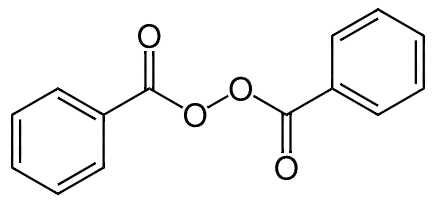
\includegraphics[scale=0.3]{00Figuras/POB-removebg-preview.png}
    \caption{a) peróxido de benzoilo}
    \label{POB}
\end{figure}

\begin{figure}[H]
    \centering
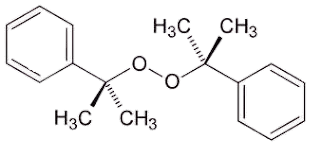
\includegraphics[scale=0.4]{00Figuras/PUC.png}
    \caption{b) peróxido de cumilo}
    \label{PUC}
\end{figure}


\section{Caracterización}



\textbf{Probetas:} 20 gramos de caucho molido de llanta y sobre eso se agrega 2\% del iniciador peróxido de benzoilo.

\textbf{Prensa:} Se utilizó la prensa hidráulica de 15 toneladas modelo MEGA KSC-15A, equipada con la bomba XX, para realizar la compresión de las probetas.

z

\section{Equipos}

Los equipos que se mencionan a continuación se utilizaron para caracterizar el material GTR original, así como las mezclas de GTR con agente desvulcanizante antes y después de la radiación con microondas. Esto permitió observar las características iniciales del material recibido, su composición, la cual influye en los resultados de la reacción, y evidenciar y comparar los posibles cambios ocurridos en los enlaces.


\subsection{Análisis termogravimétrico (TGA)}
Se utilizó un equipo TGA (Análisis Termogravimétrico) de Mettler Toledo para analizar los cambios de masa de la muestra en un rango de temperaturas de XX °C a XX °C, bajo una atmósfera inerte de XX a un flujo de XX mL/min y con una rampa de calentamiento de XX °C/min.

\begin{figure}[H]
    \centering
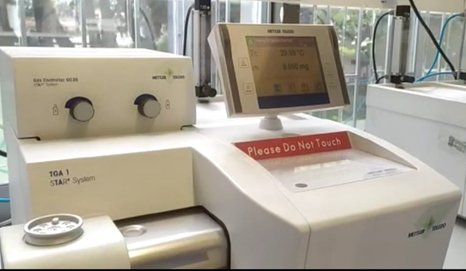
\includegraphics[scale=0.55]{00Figuras/TGA.png}
    \caption{\hl{Equipo TGA}}
    \label{TGA}
\end{figure}

\subsection{Calorimetría diferencial de barrido (DSC) }
Se utilizó un calorímetro diferencial de barrido (DSC) modelo \hl{HP DSC 1 STAR System} Mettler Toledo para analizar las propiedades térmicas de la muestra. Las mediciones se realizaron en un rango de temperaturas de xx °C a XX °C, bajo una atmósfera de XX a un flujo de XX mL/min. La muestra fue sometida a una tasa de calentamiento de XX °C/min. %Durante el análisis, se registraron las siguientes transiciones térmicas: \hl{explicar cuales se evidenciaron}

\begin{figure}[H]
    \centering
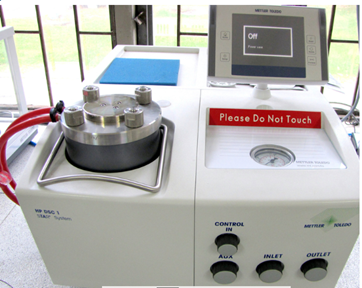
\includegraphics[scale=0.6]{00Figuras/DSC.png}
    \caption{\hl{Equipo DSC}}
    \label{DSC}
\end{figure}

\subsection{Espectroscopía infrarroja por transformada de Fourier (FTIR)}

La espectroscopía infrarroja por transformada de Fourier (FTIR) utilizando la técnica de XX se llevó a cabo con una resolución de XX \unit{cm^{-1}} y XX escaneos, en un rango de número de onda de XX a XX \unit{cm^{-1}}. Esta técnica se aplicó a las muestras que presentaron los mayores cambios en sus propiedades físicas durante el proceso de desvulcanización por microondas. Se anticipan modificaciones en los picos del espectro asociados a los enlaces S-S (565 \unit{cm^{-1}}) y C-S (XX \unit{cm^{-1}}).  

%Texto de prueba a ver qué tan bonito se ve.

%Segundo texto de prueba, se necesita probar mucho een esta vida.


\subsection{Reómetría}

Se utilizó un reómetro para medir las propiedades reológicas del caucho, modelo XX.

\subsection{Microondas-Magnetrón}

\section{Reacción}

\subsection{Microondas}

\begin{figure}[H]
    \centering
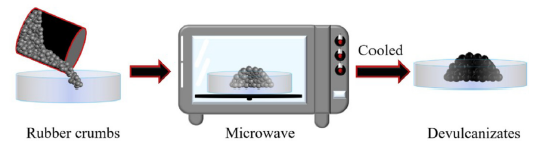
\includegraphics[scale=0.6]{00Figuras/microwave.png}
    \caption{\hl{TERMINAR DE MODIFICAR IMAGEN PROPIA DE ESTA}}
    \label{PUC}
\end{figure}

\end{multicols}


% \end{multicols}


